\section*{Aufgabe 1: Passendes Vorgehensmodell für große Projekte}

Die Auswahl des Vorgehensmodells ist essentielle für Projekte, da diese unterschiedliche Vor- und Nachteile bieten. Verschiedene Modelle haben andere Anforderungen an das Team, dessen Struktur sowie die Erfahrung der Mitglieder und deren Selbstorganisation. Außerdem beeinflussen diese das Produkt, welches ausgeliefert wird und wann beziehungsweise wie es ausgeliefert wird.

Sofern die Anforderungen eines Projektes vollständig bekannt und als stabil beziehungsweise als unveränderlich angenommen werden können, eignet sich das Wasserfallmodell. Es handelt sich um ein lineares und vorhersehbares Verfahren, dadurch ist es gut geeignet in stark regulierten Umgebungen und Situationen in denen eine ausgiebige Dokumentation notwendig ist.
Das Wasserfallmodell legt dabei feste zeitliche Abläufe und Fristen fest. Es ist dabei weniger auf Zusammenarbeit zwischen den Teams ausgelegt, da es sehr hierarchisch strukturiert ist und die Abläufe fest, folgend aufeinander, definiert sind.
Das Produkt wird beim Wasserfallmodell am Ende ausgeliefert, was Rückmeldungen erst sehr spät erlaubt. Außerdem verhindert es frühzeitig auf Änderungswünsche eingehen zu können.

Scrum eignet sich für komplexe Projekte, dessen Anforderungen noch nicht vollständig eindeutig sind. Es erlaubt dabei jedoch die inkrementelle Verbesserung des Produktes. Dazu arbeitet Scrum in festgelegten zeitlichen Perioden, den Sprints.
Scrum fördert dabei die Zusammenarbeit unter Teams durch Austausch in Daily Standups und Sprint Retrospektiven. Das Arbeiten in Sprints erlaubt eine Auslieferung des Produktes beziehungsweise Inkrementen dessen. So kann Feedback früh gesammelt und einen Einfluss auf die Entwicklung haben.

Kanban erlaubt ebenfalls die kontinuierliche Verbesserung beziehungsweise Abarbeitung von Items, ist jedoch nicht auf fest vorgelegte zeitliche Perioden beschränkt. Es erlaubt dadurch Flexibilität und fokussiert sich auf Lead Time und Cycle Time und zeigt damit Bottlenecks auf. Dadurch kann es die Arbeit effizienter machen.
Kanban erfordert jedoch ein Team, welches sich gut selbst organisiert.

\section*{Aufgabe 2: Angepasste Stacey-Matrix}

\subsubsection*{Simple: Auslieferung von Template-Produkten}

Es wird auf einen eigenes Website-Template zurückgegriffen, das nur leicht auf den Kunden angepasst werden muss. Die Anforderungen sind klar und wiederholen sich über verschiedene Kunden ebenfalls, z.B. Logo- und Corporate Identity des Kunden hinzufügen. Dies lässt sich sehr leicht standardisieren und entsprechend in Prozessen abarbeiten und später überprüfen.

\subsubsection*{Complicated: Skalierung einer Datenbank-Architektur}

Die Skalierung einer Datenbank auf ein festgelegtes Ziel an Requests/Zeit gilt als \gq{Complicated}, da das Ziel wohldefiniert ist. Jedoch ist die technische Lösung noch nicht geklärt. Es stehen verschiedene Optionen zur Verfügung (z.B. vertical scaling, sharding, read replicas), welche gegeneinander abgewogen werden müssen.

\subsubsection*{Complex: Entwicklung einer KI-Chatbot-App}

Das Ziel ist eindeutig, jedoch verbleiben Punkte welche geklärt werden müssen. Es ist zum Beispiel noch nicht klar, wie die Architektur aussehen wird um eine variable Anzahl an Nutzern zu verarbeiten. Es ist ebenfalls zu klären, welches KI-Modell verwendet wird, dies hat Auswirkungen auf die benötigte Rechenleistung und beeinflusst die Zufriedenheit der Nutzer.

\subsubsection*{Chaotic: Systemausfall}

Die Situation ist meist chaotisch, Anforderungen und Lösungswege sind zunächst nicht klar, da der Grund für den Ausfall erstmal nicht genau bestimmt werden kann. Ziel ist vorerst den Ausfall zu beheben durch Alternativpläne oder Notfalllösungen. Danach kann analysiert und geplant werden, diesen Ausfall aufzuarbeiten.

\section*{Aufgabe 3: Scrum}

\subsubsection*{3.1:}

User Story \#2 \gq{Film oder Serie zufällig abspielen}

\textbf{User Story 3.1 - 2 Story Points:} \gq{Als Nutzer möchte ich einen zufälligen Film/Serie aus dem gesamten Katalog abspielen.}\\
\textbf{User Story 3.2 - 3 Story Points:} \gq{Als Nutzer möchte ich einen zufälligen Film/Serie aus meiner Liste abspielen.}\\
\textbf{User Story 3.3 - 3 Story Points:} \gq{Als Nutzer möchte ich auswählen können, ob ich einen Film, eine Serie oder eins von beidem zufällig abspielen möchte.}

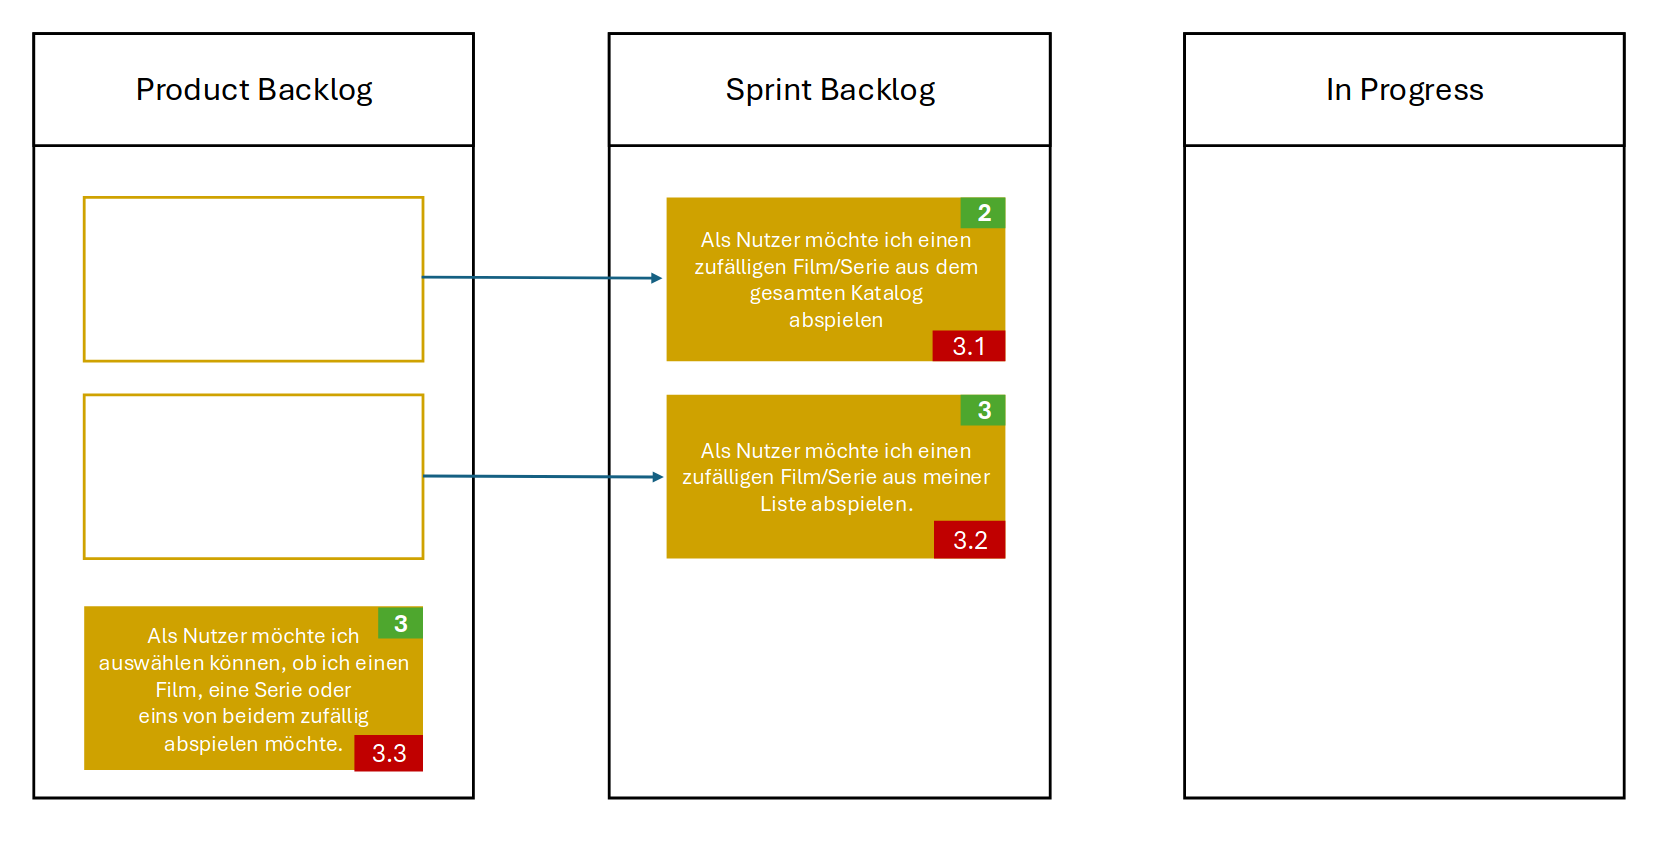
\includegraphics[width=\textwidth]{images/UE3_3.1.png}

\subsubsection*{3.2:}

Akzeptanzkriterien sind Bedingungen, die es zu erfüllen gilt, damit ein Item / eine User Story als abgeschlossen gilt. Sie dienen als klare, überprüfbare Definition vom \gq{Fertig}-Status. Sie werden definiert, damit das Team eine transparente Definition hat und helfen bei der Testbarkeit / Überprüfbarkeit bei Abschluss des Items.

\textbf{User Story 3.1:}
\begin{itemize}
\item Knopf zum Aufrufen der Zufalls-Schaltfläche ist sichtbar auf der Hauptseite.
\item Knopf besitzt ein eindeutiges Icon.
\item Der Knopf ist klickbar, ruft Zufalls-Schaltfläche korrekt auf und erlaubt einen zufälligen Film oder Serie abzuspielen.
\end{itemize}
\textbf{User Story 3.2:}
\begin{itemize}
\item Zufalls-Schaltfläche besitzt eine Option zur Auswahl zwischen allen oder gespeicherten Titeln in der eigenen Liste.
\item Schaltfläche reagiert visuell auf Input, hebt aktuell gewählte Option deutlich vor.
\item Bei Klick wird ein Film/Serie basierend auf Auswahl gestartet.
\end{itemize}
\textbf{User Story 3.3:}
\begin{itemize}
\item Zufalls-Schaltfläche besitzt eine Option zur Auswahl zwischen Serien, Filmen oder beidem.
\item Schaltfläche reagiert visuell auf Input, hebt aktuell gewählte Option deutlich vor.
\item Die Schaltfläche ist klickbar, reagiert visuell bei Interaktion und spielt einen zufälligen Film, Serie oder eins von beidem ab.
\end{itemize}

\subsubsection*{3.3:}

\textbf{User Story 3.1:} Simple, da die Anforderung und Lösungen klar sind. Es handelt sich um eine einfach einzublendende UI, sowie ein simpler Zufallsalgorithmus zum Abspielen der Inhalte.\\
\textbf{User Story 3.2:} Complicated - technische Umsetzung geht über Zufallsalgorithmus hinaus. Nun werden Daten und deren Abruf benötigt, welche Inhalte der Nutzer gespeichert hat. Die Schaltfläche muss um einen 2-Way Switch erweitert werden.\\
\textbf{User Story 3.3:} Complicated - nur leicht komplizierter als 3.2, Anforderungen gestalten sich ähnlich. Es werden zusätzlich Daten benötigt, welcher Inhalt als Film oder Serie klassifiziert wird. Zusätzlich benötigt die UI einen 3-Way Switch um drei Optionen auswählbar zu machen.